\documentclass[12pt]{article}
\def\activityid{F05-K-v3}\usepackage[letterpaper,margin=.65in,top=.60in,bottom=.65in]{geometry}
\usepackage[T1]{fontenc}\usepackage[default]{sourcesanspro}
\usepackage{microtype,tikz,array,tabularx,fancyhdr,amsmath}\usepackage[hidelinks]{hyperref}
\usetikzlibrary{arrows.meta,calc}
\setlength{\parindent}{0pt}\setlength{\parskip}{7pt}\setlength{\headheight}{0pt}\setlength{\footskip}{26pt}\setlength{\emergencystretch}{2em}
\pagestyle{fancy}\fancyhf{}\renewcommand{\headrulewidth}{0pt}\renewcommand{\footrulewidth}{.4pt}
\fancyfoot[L]{\scriptsize Bellingham Math Circle / Week 5 / \activityid}\fancyfoot[R]{\scriptsize \thepage}
\definecolor{ink}{gray}{.12}\definecolor{soft}{gray}{.95}\color{ink}
\newcommand{\PageTitle}[2]{{\fontsize{10}{12}\selectfont\bfseries WEEK 5\quad TOWER LAB\hfill #1\par}\vspace{3pt}{\fontsize{26}{29}\selectfont\bfseries #2\par}\vspace{2pt}}
\newcommand{\Subhead}[1]{\par\vspace{3pt}{\large\bfseries #1}\par}
\newcommand{\RuleBox}[1]{\par\begingroup\setlength{\fboxsep}{8pt}\colorbox{soft}{\parbox{\dimexpr\linewidth-16pt\relax}{#1}}\endgroup\par}
\newcommand{\WriteBox}[2]{\par\textbf{#1}\par\vspace{2pt}\begin{tikzpicture}\draw[black!40,line width=.5pt] (0,0) rectangle (\dimexpr\linewidth-.5pt\relax,#2);\end{tikzpicture}\par}
\newcommand{\Code}[1]{\texttt{#1}}

\newcommand{\StudentHeader}[1]{{\fontsize{10}{12}\selectfont\bfseries Week 5 / Tower lab / #1\par}\vspace{10pt}}
\newcommand{\Problem}[2]{\par\vspace{4pt}\textbf{Problem #1:} #2\par}
\newcommand{\RecordBox}[2]{\par #1\par\vspace{2pt}\begin{tikzpicture}\draw[black!40,line width=.5pt](0,0)rectangle(\dimexpr\linewidth-.5pt\relax,#2);\end{tikzpicture}\par}

\hypersetup{pdftitle={Week 5: K--1}}
\begin{document}
\StudentHeader{K--1}
\Problem{1}{Use towers of heights 1, 2, and 3. Put them in the order 2, 1, 3 from left to right. Look from the left, then the right. A taller tower hides a shorter one behind it. Write 2, 1, 3 from left to right in both rows below. Circle the towers you see from each end.}
\begin{center}\begin{minipage}{.48\linewidth}\centering Looking from the left\\[8pt]\begin{tikzpicture}[x=.6in,y=.6in]\draw[step=1,black!55](0,0)grid(3,1);\node[left]at(-.15,.5){left};\node[right]at(3.15,.5){right};\end{tikzpicture}\end{minipage}\hfill\begin{minipage}{.48\linewidth}\centering Looking from the right\\[8pt]\begin{tikzpicture}[x=.6in,y=.6in]\draw[step=1,black!55](0,0)grid(3,1);\node[left]at(-.15,.5){left};\node[right]at(3.15,.5){right};\end{tikzpicture}\end{minipage}\end{center}
\Problem{2}{Rearrange the towers into 1, 3, 2. Look from both ends again. Draw or write the tower heights. Circle the towers you see.}
\begin{center}\begin{minipage}{.48\linewidth}\centering Looking from the left\\[8pt]\begin{tikzpicture}[x=.6in,y=.6in]\draw[step=1,black!55](0,0)grid(3,1);\node[left]at(-.15,.5){left};\node[right]at(3.15,.5){right};\end{tikzpicture}\end{minipage}\hfill\begin{minipage}{.48\linewidth}\centering Looking from the right\\[8pt]\begin{tikzpicture}[x=.6in,y=.6in]\draw[step=1,black!55](0,0)grid(3,1);\node[left]at(-.15,.5){left};\node[right]at(3.15,.5){right};\end{tikzpicture}\end{minipage}\end{center}
\Problem{3}{Rearrange the same three towers for each view below. Draw or write each row from left to right.}
\begin{center}\renewcommand{\arraystretch}{2.8}\begin{tabular}{p{2.8in}|p{2.8in}}Towers seen from the left & My tower order\\\hline
3 & \\
1 & \\
2 & \\\end{tabular}\end{center}

\newpage
\StudentHeader{K--1}
\Problem{4}{Build different rows with heights 1, 2, and 3. Keep the left end in the same place. Record each new order and count the towers seen from each end. Do not record the same order twice.}
\begin{center}\renewcommand{\arraystretch}{3.0}\begin{tabular}{c|p{2.5in}|c|c}Row & Tower order, left to right & Seen left & Seen right\\\hline
1 &  &  & \\
2 &  &  & \\
3 &  &  & \\
4 &  &  & \\
5 &  &  & \\
6 &  &  & \\\end{tabular}\end{center}
\Problem{5}{Compare your recorded rows. Circle the rows that show two towers from the left and two from the right. Build each circled row again and check both views.}
\RecordBox{A row I checked:}{1.1in}

\newpage
\StudentHeader{K--1}
\Problem{6}{Try to make a row of heights 1, 2, and 3 that shows only one tower from each end. Record two different attempts. For each attempt, count from both ends.}
\begin{center}\renewcommand{\arraystretch}{2.7}\begin{tabular}{p{3in}|c|c}Tower order & Seen left & Seen right\\\hline
 &  & \\
 &  & \\\end{tabular}\end{center}
\Problem{7}{Make a tiny city using two towers of height 1 and two of height 2. Put one tower in each square. Every row and every column must contain both heights. Record two different cities. Circle the city whose top row shows two towers from the left.}
\begin{center}\begin{minipage}{.48\linewidth}\centering 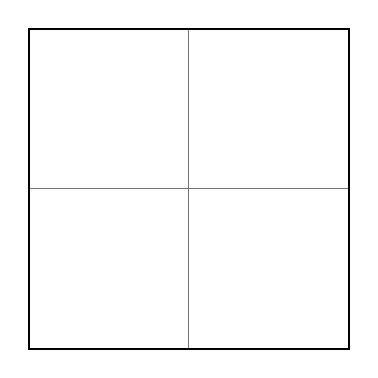
\begin{tikzpicture}[x=0.8in,y=0.8in]\draw[step=1,black!55](0,0)grid(2,2);\draw[thick](0,0)rectangle(2,2);\end{tikzpicture}\end{minipage}\hfill\begin{minipage}{.48\linewidth}\centering 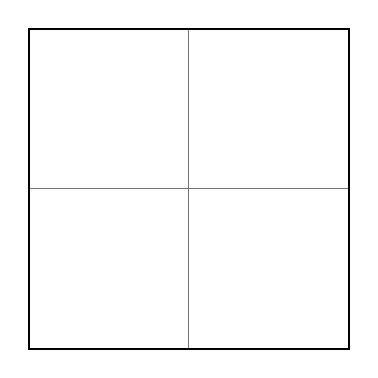
\begin{tikzpicture}[x=0.8in,y=0.8in]\draw[step=1,black!55](0,0)grid(2,2);\draw[thick](0,0)rectangle(2,2);\end{tikzpicture}\end{minipage}\end{center}

\end{document}
